\section{Ergebnisse}
\subsection{Physische Risiko}
Das erstellte Portfolio umfasst 3853 Datenpunkte.Die Hochwasserrisikostufen sind wie folgt verteilt: 1 hohes, 17 mittlere, 12 niedrige und 3823 sehr niedrige Risiken. Diese Risikostufeverteilung wird in Abbildung \ref{fig:riskostufe} graphisch dargestellt und visualisiert.
\begin{figure}[htbp]
    \centering
    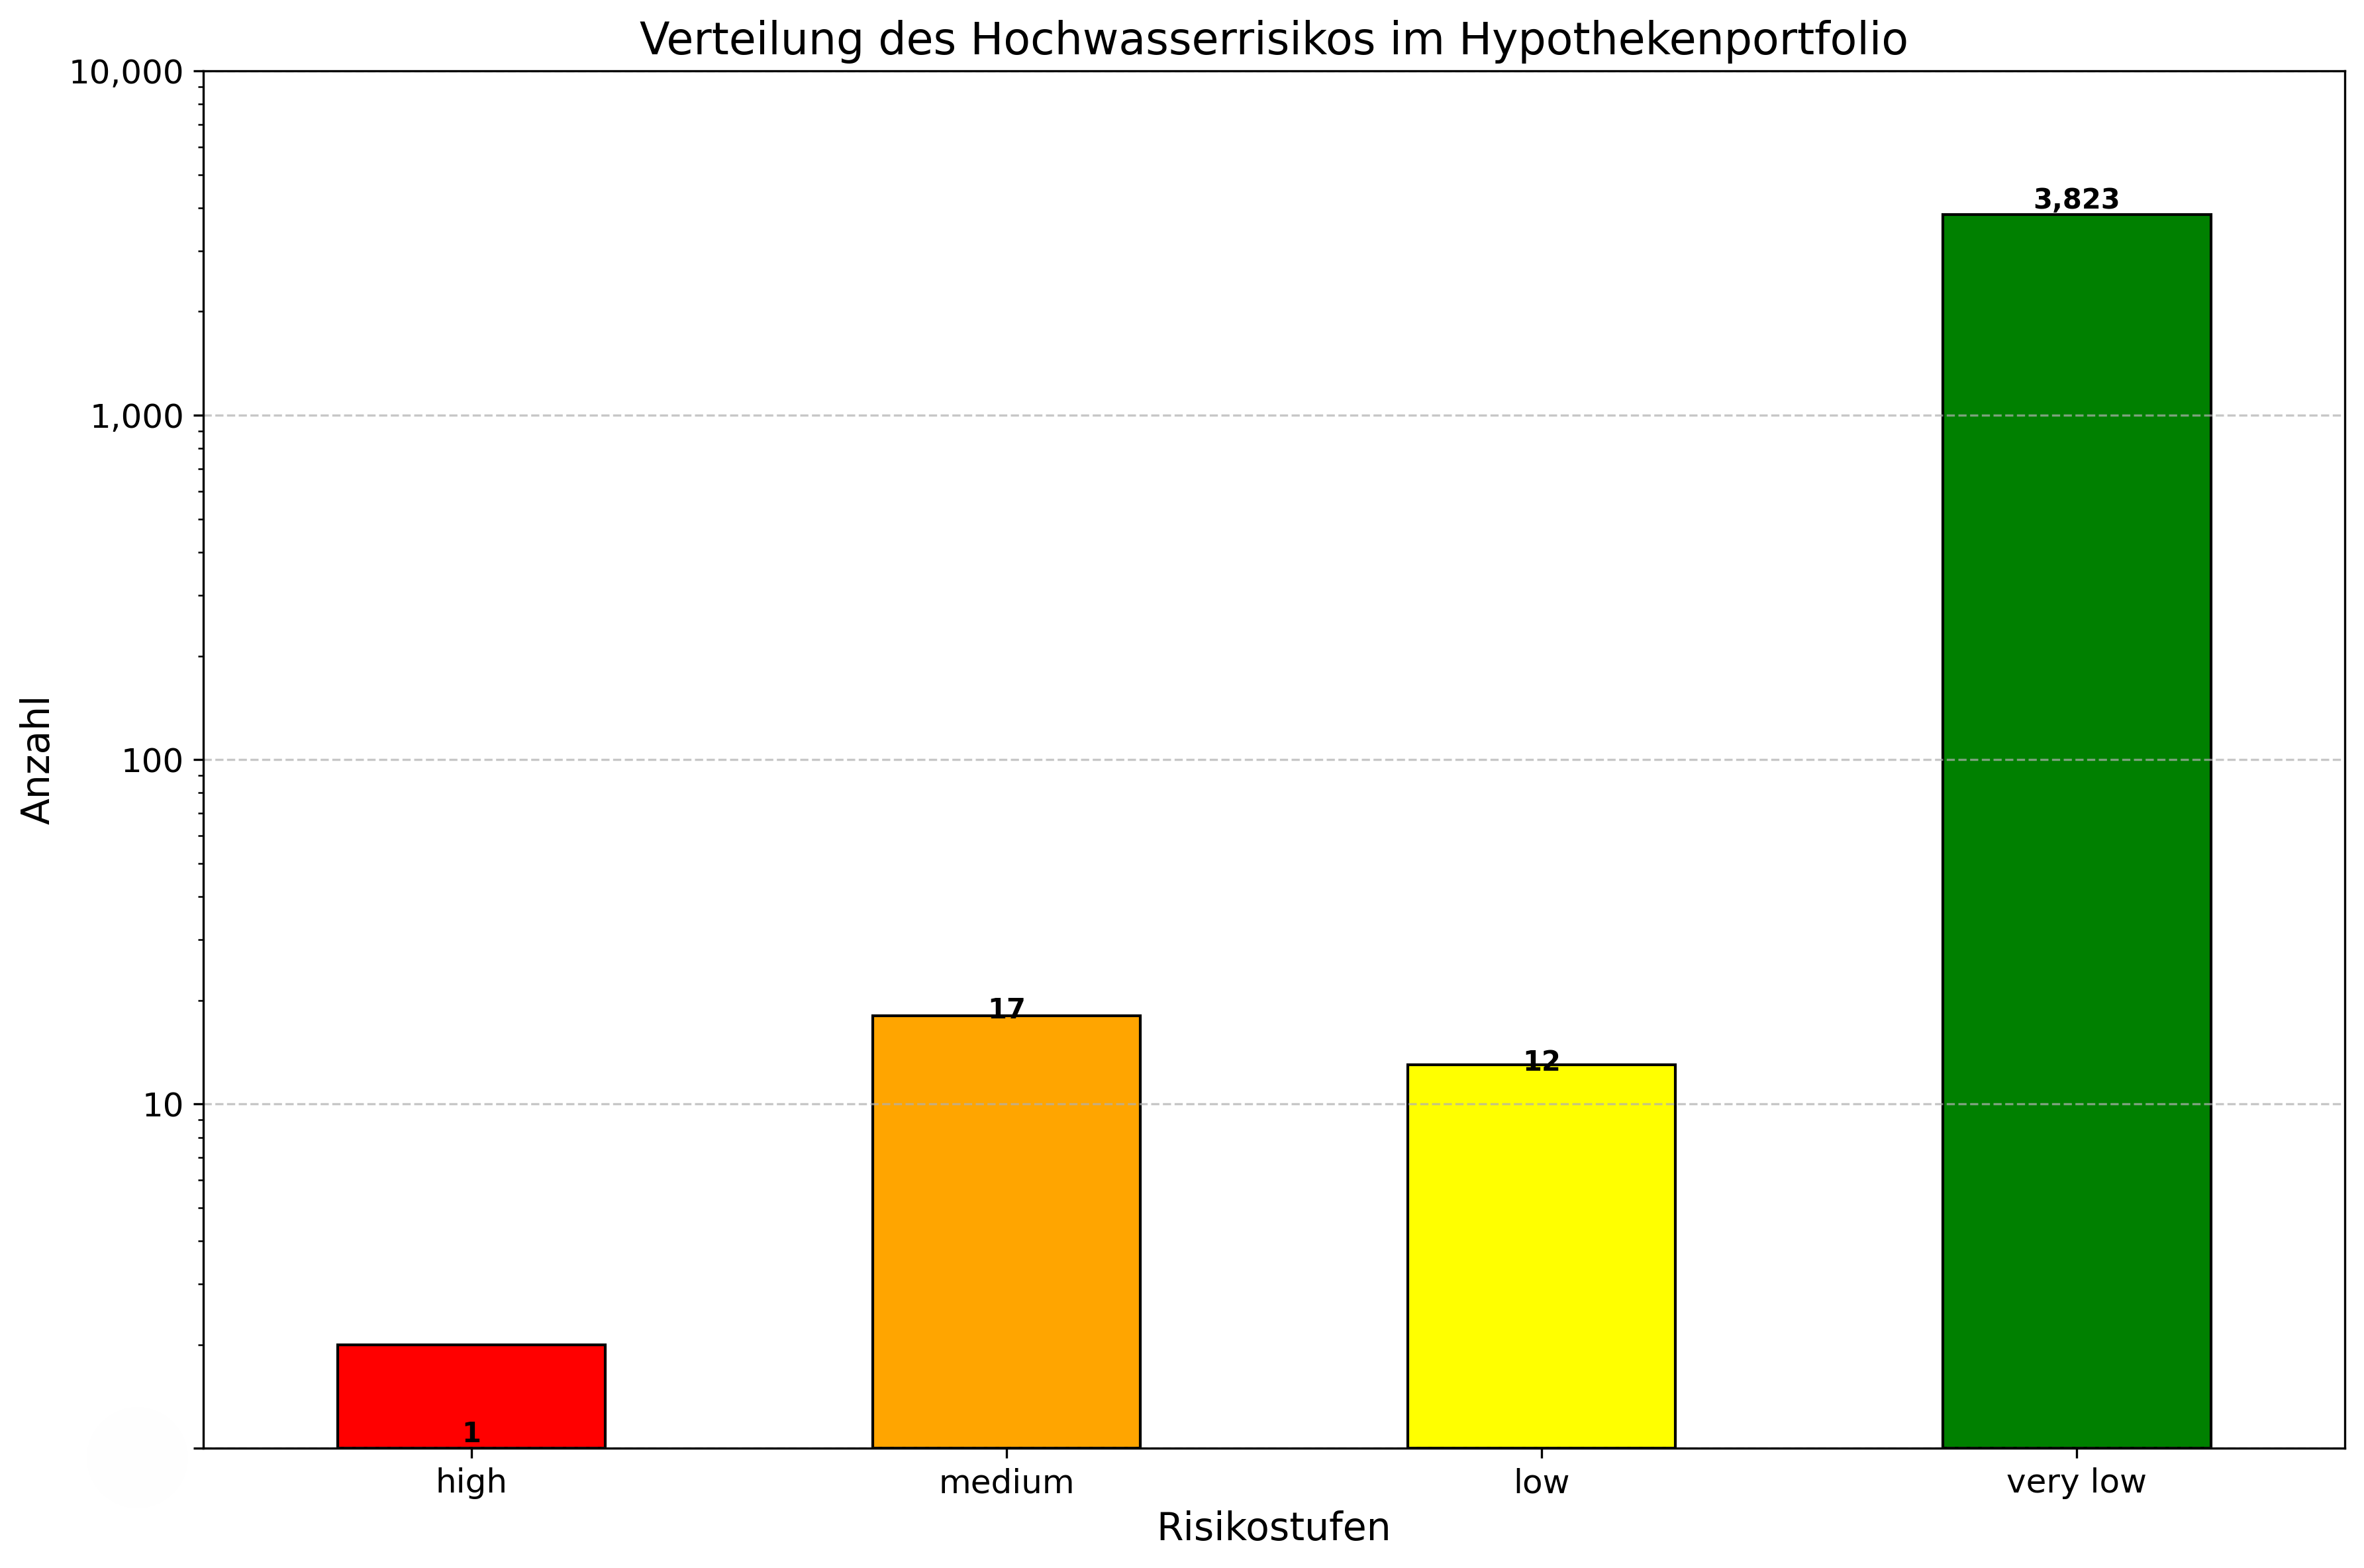
\includegraphics[width=\textwidth]{figures/hochwasserrisiko_verteilung.png}
    \caption{Verteilung der Hochwasserrisikostufen im m Hypothekenportfolio. Quelle: Eigene Darstellung}
    \label{fig:riskostufe}
\end{figure}
\FloatBarrier
Mittels des digitalen Geländemodells von Bayerns sowie Pegelnullpunkt und Hochwasserstand von \textcite{bayern2016hochwassernachrichtendienst} wurde die Überflutungstiefe bestimmt. Dies betrifft Datenpunkte in den Kategorien hoch, mittel und niedrig.
Aufgrund der Größe der \ac{DGM}-Daten (240 GB) erfolgte die Berechnung nur für 30 Punkte in Hochrisiko-, mittlerem und niedrigem Risikogebiet. Entsprechende Orts-, Gemeinde- und Landkreisdaten wurden geladen.
Im Hochrisikogebiet liegt ein einzelner Punkt in Haag an der Amper. Dort beträgt die maximale Überflutungstiefe 2,1 m, entsprechend einem Schadensfaktor von 0,16.
17 Datenpunkte befinden sich in Gebieten mittleren Risikos, verteilt auf verschiedene Orte.In der Kategorie mittleres Risiko gibt es Punkte mit einer Überschwemmungstiefe von 0. Dies ist durchaus plausibel. Innerhalb eines Gebiets mit mittlerem Risiko variiert die Topographie. Höher gelegene Standorte weisen eine geringere Überflutungstiefe auf. Ähnlich verhält es sich mit Datenpunkten in Gebieten mit niedrigem Risiko. Auch dort können nicht-null Überschwemmungstiefen auftreten. Dies ist auf die niedrigere Geländehöhe zurückzuführen. 

Die Ermittlung der Tiefe für 3823 Datenpunkte in sehr niedrigen Risikogebieten wurde nicht durchgeführt. Diese Datenpunkte umfassen 1518 Orte, verteilt über 72 Landkreise.Eine individuelle Bewertung wäre äußerst aufwendig, da nicht nur das manuelle Laden aller Kartendaten erforderlich wäre, sondern auch kein umfassender Datensatz für Bayern mit Pegelnullpunkten und Hochwasserständen aller Orte existiert. Aufgrund dieser Einschränkungen wurde für alle Datenpunkte in sehr niedrigen Risikogebieten eine Überflutungstiefe von 0 angenommen.